%\chapter{\label{results}Two-body decay kinematics}

%\setcounter{equation}{0}
%\setcounter{table}{0}
%\setcounter{figure}{0}
%\baselineskip 24pt
%\hspace{10pt}
%\\
\section{Kinematics}
\subsection{Four momentum}
\noindent
\begin{itemize}
    \item 
Relativistic kinematics problems are greatly simplified by using $4-$vectors,
for any $4-$momentum $p^{\mu}$ is given by,

\begin{equation}
    p^{\mu} = (E/c, \Vec{p})= (m\gamma c, m \gamma \Vec{u})
\end{equation}
\item
A four momentum equation automatically takes into account conservation of energy and momentum. For example, if a particle $X$ decays into two daughters,
we write the $4-$momentum equation will be
\begin{equation}
  P_{X}^\mu = p_{a}^\mu + p_{b}^\mu  
\end{equation}
\item Where the mass $M$ of the heavier particle is given by $p_{0}.p_{0}=M^2c^2$. By measuring the energy and momentum of the daughter particles, one can reconstruct the invariant mass of the two-particle system, which must be equal to $M$.
\end{itemize}
   
%%%%%%%%%%%%%%%%%%%%%%%%%%%%%%%%%%%%%%%%%%%%%%%%%%%%%%%%%%%%%%%%%%%%%%%%%%%%%%%%

\subsection{Particle decay in Center of mass frame}
Consider the decay of a particle$(X)$ with mass $M$ to two particles of mass $m_{a}$ and $m_{b}$ in the rest frame of the parent particle. 
Application of $4-$momentum conservation leaves us with just $2$ degrees of freedom. Two daughter particles must be emitted back
to back in the parent rest frame for conserving momentum.
\begin{figure}[h]
    \centering
    \includegraphics[width = 9cm, height = 5.5cm]{cm3.png}
    \caption{Particle decay in CM-frame}
    \label{fig:my_label}
\end{figure}
\hspace{10pt}
\\
\begin{itemize}
    \item 
In CM frame for $a$ and $b$ mother particle $X$ is at rest, so the $4-$momenta will be 
        \begin{equation}
            \textbf{p}_{X} = (M c,0,0,0), \textbf{p}_{a}= (E_{a}/c, \Vec{p}_{a}), \textbf{p}_{b}= (E_{b}/c, \Vec{p}_{b})
        \end{equation}
\item        
 Conservation of $4-$momentum requires the following 
\begin{equation}
    \textbf{p}_{X} = \textbf{p}_{a} + \textbf{p}_{b} \implies \Vec{p}_a = -\Vec{p}_b
\end{equation}    
        
\item    
 For energy conservation 
 \begin{equation}
     E_{a}+E_{b} = \sqrt{m_{a}^2c^4+p^2c^2}+ \sqrt{m_{b}^2c^4+p^2c^2} =M c^2
 \end{equation}

\end{itemize}

By solving the above relation we got the expression 
        \begin{equation}
            p = c\frac{\sqrt{[M^2-(m_{a}-m_{b}^2)][M^2-(m_a +m_b)^2]}}{2M}
        \end{equation}

Which results  
    \begin{equation}
         M \geq m_{a} + m_{b}
    \end{equation}

So, if the particle has greater mass than sum of masses of two daughter particles
particle is unstable and decays.  Momenta of daughter particles and energies fixed by $3$ masses
from energy conservation $E_{b}=\sqrt{E_{a}^2-m_{a}^2c^4+m_{b}^2c^4}$ solve to get that 
        \begin{equation}
            E_{a} = \frac{(M^2+m_{a}^2-m_{b}^2)c^{2}}{2M}
        \end{equation}
    similarly
        \begin{equation}
            E_{b} = \frac{(M^2+m_{b}^2-m_{a}^2)c^{2}}{2M}
        \end{equation}
There is no preferred direction in which the daughter particles travel. So decay is said to be isotropic in which daughter particles traveling back-to-back in $X$ rest frame.

%%%%%%%%%%%%%%%%%%%%%%%%%%%%%%%%%%%%%%%%%%%%%%%%%%%%%%%%%%%%%%%%%%%%%%%%%%%%%%%%%%%

\subsection{Particle decay in Lab frame}
Previously, we have determined energy and momentum  for two-body decay in the parent particle CM frame. However, we need to find their values in the frame where the parent particle is moving, e.g. the detector frame(Lab frame).  
\begin{figure}[h]
    \centering
    \includegraphics[width=11cm, height=5cm]{lab3.png}
    \caption{Particle decay in Lab-frame}
    \label{fig:my_label}
\end{figure}
\\
\noindent
\begin{itemize}
    \item 
By taking  $\hat{z}$-axis along direction of flight of mother particle, the $4-$momenta for  $a$, $b$ and  mother particle $X$ is at lab frame will be 
        \begin{equation}
            \textbf{p}_{X} = (E/c,0,0,p), \textbf{p}_{a}= (E_{a}/c, \Vec{p}_{a\perp}, p_{a z}), \textbf{p}_{b}= (E_{b}/c, \Vec{p}_{b\perp}, p_{b z})
        \end{equation}
\item        
By momentum conservation (transverse momentum vectors)
        \begin{equation}
            \Vec{p}_\perp \equiv \Vec{p}_{a\perp} =  -\Vec{p}_{b\perp} 
        \end{equation}
\item
Energies and $\hat{z}$ components of particle momenta
related to those in the CM-frame by a Lorentz boost
with a boost velocity equal to the speed of the mother particle along $\hat{z}$ direction is given by         
    \begin{equation}
    \begin{split}
                E_{a} =& \gamma (E^{*}_a/c + \beta p^{*}_{a z})\\
                p_{a z} =& \gamma (p^{*}_{a z}+\beta E_{a}^{*}/c)\\
                \Vec{p}_{a\perp} =& \Vec{p}_{a\perp}^{*}\\
    \end{split}
    \end{equation}
similarly for $b$ particle, 
    \begin{equation}
    \begin{split}
                E_{b} =& \gamma (E^{*}_b/c + \beta p^{*}_{b z})\\
                p_{b z} =& \gamma (p^{*}_{b z}+\beta E_{b}^{*}/c)\\
                \Vec{p}_{b\perp} =& \Vec{p}_{b\perp}^{*}\\
                \beta = p c/ E  \  \ &and  \ \ \gamma = E/ (M c^{2}) 
    \end{split}
    \end{equation}
\end{itemize}

\noindent    
This completely solves problem
from which we can find angles $(\theta)$ which daughter particles
make with $z$-axis and with each other as functions of $p_{X}$.

\begin{figure}[h]
    \centering
    \includegraphics[width=12cm, height=4cm]{1.png}
    \caption{Comparison between CM frame$(S)$ and Lab frame$(S^\prime)$}
    \label{fig:my_label}
\end{figure}
\begin{itemize}
    \item 
In $S$ frame(Rest frame) four momentum is given by  
    \begin{equation}
        p^{\mu} = (E/c, p \cos{\theta}, p\sin{\theta}, 0)
    \end{equation}
\item
In $S^{\prime}$(boosted frame) it follows as 
    \begin{equation}
        p^{\prime\mu} = (E^\prime/c, p^\prime \cos{\theta^\prime}, p^\prime\sin{\theta^\prime}, 0)
    \end{equation}
\end{itemize}
\noindent

Applying $S \longrightarrow S^{\prime}$ Lorentz transformation
\begin{equation}
    \begin{split}
        p^{\prime}\cos{\theta^{\prime}} = & \gamma^{*}(p\cos{\theta}-\beta^{*}E/c)\\
        p^{\prime}\sin{\theta} =& p\sin{\theta}
    \end{split}
\end{equation} 
So 
\begin{equation}
    \begin{split}
        \tan {\theta^{\prime}} =& \frac{p\sin{\theta}}{\gamma^{*}(p\cos{\theta}-\beta^{*}E/c)} \\
        \implies tan\theta^{\prime} =& \frac{\sin{\theta}}{\gamma^{*}(\cos{\theta}-\beta^{*}/\beta)}\label{eq:3.17}
    \end{split}
\end{equation}
\\ 
where $\beta^{*} = v/c$ is velocity of $S$ wrt $S^{\prime}$ and $\beta= p c/E$ is velocity of particle in $S$ frame .\\

\begin{figure}[h]
    \centering
    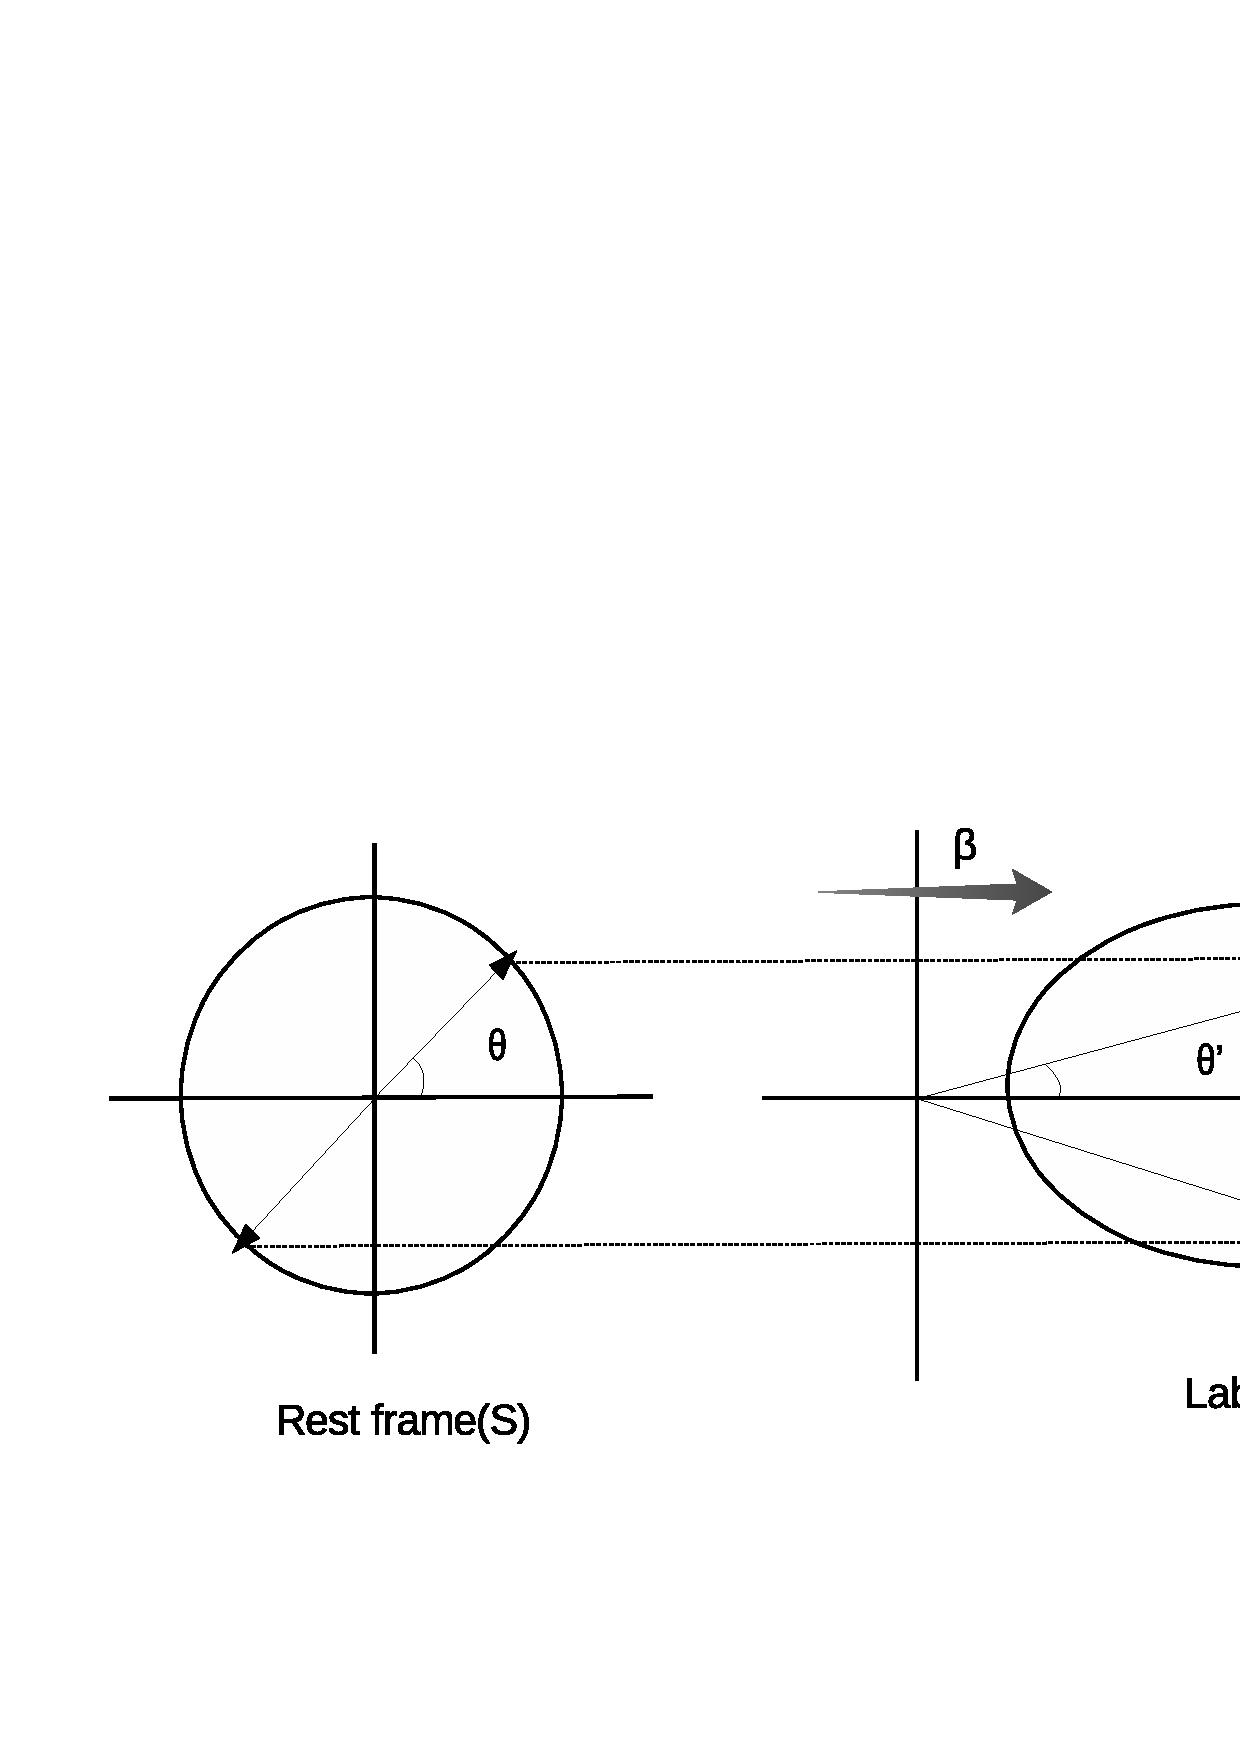
\includegraphics[width=12cm, height=8cm]{3.png}
    \caption{Transformation from $S$ frame to $S^{\prime}$ frame}
    \label{fig:my_label}
\end{figure}
%%%%%%%%%%%%%%%%%%%%%%%%%%%%%%%%%%%%%%%%%%%%%%%%%%%%%%%%%%%%%%%%%%%%%%%%%
\subsection{Invariant Mass}
Invariant mass is useful to find mass of short-live unstable particles from momenta of their observed decay product(e.g $Z\longrightarrow \mu^{+}\mu^{-} \ \ or \ \ e^{+}e^{-} $).

\begin{itemize}
\item 
The invariant mass of a system consisting of $N$ particles is defined as the norm of its total momentum four-vector 
\begin{equation}
    m = \left|\sum_{i=1}^N p_{i}\right|
\end{equation}
\item
Consider $X\longrightarrow a+b$ process, by momentum conservation one can write 
$p_{x} = p_{a}+ p_{b}$, which gives the relation 
\begin{equation}
\begin{split}
        m^2_X c^{2} =& \ \ (p_{a}+p_{b})^2\\
        =&\ \  p_{a}^2 + p_{b}^2 + 2p_{a}.p_{b}\\
        =&\ \  m_{a}^2c^2 + m_{b}^2c^2 + 2E_{a}E_{b}/c^2 -2\Vec{p}_{a}.\Vec{p}_{b}
\end{split}
\end{equation}
\end{itemize}
